\section{History placement when a prefix changes area}
\label{sec:sb-prefix}
The position of a history record determines which prefixes an instruction
replaces and when its scans terminate. If it replaces prefixes of lengths
$a,b$ by prefixes of lengths $a',b'$, its planar determinant contains
$B^{a+b-a'-b'}$, where $B$ is the radix. The following processors retain
these length changes explicitly and use the geometric tools already proved.
Our goal is the family of fixed-label halting events stated in
Theorem~\ref{thm:sb-realizations} below. We first prove the symbolic
instructions, then realize their full branch domains in
Section~\ref{sec:sb-geometry}, and finally verify initialization and
continuous-time observation in Section~\ref{sec:sb-events}.

Two geometric conclusions will be useful. A compensating third scale
realizes the instruction on a three-dimensional neighborhood. Alternatively,
a planar field can be lifted to an incompressible field with an invariant
coding plane; only the motion in that plane is then prescribed. We will
keep these conclusions separate. We will also distinguish a loader used
once from a boot instruction that belongs to the repeated program.

The histories below implement different choices about where to store
the erased instruction and when to scan to it. The main configurations
and the stopping condition of each scan come before its finite table.
The inverse checks concern every allowed configuration, including those
outside an initialized computation. This is the information needed to
turn the symbolic branches into disjoint closed rectangles.

Throughout this section a machine has a finite tape alphabet $A$, blank $\square$, finite state set $Q$, initial state $q_0$, and halting states $H$.  Its tape is indexed by $\mathbb Z$, its head starts at $0$, and the finite input $w$ is written from cell $0$ rightwards.  For $q\notin H$ its table is
\[
 \delta(q,a)=(q',b,d),\qquad d\in\{-1,0,1\}.
\]
A missing transition may be replaced by a transition to a halting state, writing back the scanned symbol and staying in place.  Several halting states may be merged when convenient.  These finite changes preserve halting, including an initially halted machine.  An instruction
\[
 (s;\alpha,\beta)\longmapsto(s';\alpha',\beta')
\]
acts on every pair of infinite tails: $(s,\alpha L,\beta R)$ is sent to $(s',\alpha'L,\beta'R)$.  Empty prefixes are denoted by $\epsilon$.  Two prefixes are incompatible if they differ at a position specified by both.  Our instruction tables have separately disjoint source cylinders and image cylinders, including the control state in each cylinder.


\begin{remark}[A one-sided work tape]\label{rem:sb-one-sided}
The two-sided tape convention also implements a one-sided machine whose
left move at cell zero means staying at zero. Add a boundary bit to the
work alphabet, set it to one at cell zero and zero everywhere else,
and preserve it when writing. If a transition requests a left move
while reading boundary bit one, replace that displacement by zero;
otherwise retain its displacement. The head never visits a negative
cell. Induction gives exactly the original one-sided work configuration
after each transition, so all subsequent history compilers apply without
changing halting. This preprocessing also leaves a prescribed stay
instruction unchanged. The extra bit is a work symbol component,
independent of each compiler's history track and return marker.
\end{remark}

The theorem groups the constructions by their geometric domains. The
row names distinguish the history placement, loading, and routing
choices developed below; each row has its own fixed label and detector.
The proof is deferred to Section~\ref{sec:sb-events}, after the processor
and geometric constructions.

\begin{theorem}[Box, sheet, and invariant-plane realizations]
For every deterministic machine and finite input, and every fixed positive computable viscosity $\nu$, each row of the following table has a finite effective prescribed force $f=\mathcal F_\nu[U]$.\label{thm:sb-realizations}  The initial velocity is zero.  The force and velocity are smooth with all mixed derivatives bounded; the velocity has bounded kinetic energy.  On $\mathbb R^3$ their spatial supports lie in one compact set independent of time, allowed to depend on the finite instance.  On the unit torus both fields have spatial mean zero.  Their global solution is $(u,p)=(U,0)$. On the torus it is unique in the classical periodic class. For the Euclidean rows it is unique among smooth classical solutions with $u\in C_tH^2\cap C_t^1L^2$, $p\in C_tH^1$, and bounded $u,\nabla u$ on every finite time interval; pressure representatives differing by spatial constants have the same velocity conclusion. These are the specified cases of Lemma~\ref{lem:b-comparison}.

The material trajectory from the listed fixed label $a$ enters the listed fixed open set $O$ if and only if the machine halts.  In a torus row, the displayed interval is an arc of $\mathbb R/\mathbb Z$ and $O$ is that interval times $\mathbb T^2$.
\begin{center}\footnotesize
\begin{tabular}{llll}
Construction&Domain and fixed label $a$&Observation $O$&Period one from\\\hline
\multicolumn{4}{l}{\emph{Euclidean full boxes}}\\
Left-word boxes&$\mathbb R^3$, $(0,0,0)$&$x_1<-1$&$t=1$\\
Right-word boxes&$\mathbb R^3$, $(0,0,0)$&$x_1<-1/2$&$t=1$\\
Tagged storage&$\mathbb R^3$, $(-4,0,0)$&$(-1,2)^2\times(-1,1)$&$t=1$\\
Boot-window prisms&$\mathbb R^3$, $(-3,0,0)$&$x_1>0$&$t=0$\\
\multicolumn{4}{l}{\emph{Reserved-loader sheets}}\\
Left reserved sheets&$\mathbb T^3$, $(1/2,1/2,1/4)$&$(1/8,1/4)$&$t=0$\\
Right reserved sheets&$\mathbb T^3$, $(1/2,1/8,1/4)$&$(3/4,15/16)$&$t=0$\\
\multicolumn{4}{l}{\emph{Invariant planes}}\\
Frontier sine plane&$\mathbb T^3$, $(1/2,1/4,0)$&$(5/8,15/16)$&$t=1$\\
Previous-tag plane&$\mathbb T^3$, $(1/8,1/4,0)$&$(2/3,5/6)$&$t=0$\\
Shifted-start plane&$\mathbb T^3$, $(3/4,3/4,1/2)$&$(0,1/3)$&$t=0$\\
Separator sine plane&$\mathbb T^3$, $(1/4,1/2,0)$&$(1/2,1)$&$t=1$\\
Two-cell-frontier plane&$\mathbb T^3$, $(1/8,1/8,0)$&$(2/3,7/8)$&$t=1$\\
Zero-blank plane&$\mathbb T^3$, $(1/4,1/2,1/2)$&$(3/4,7/8)$&$t=1$
\end{tabular}
\end{center}
For the rows beginning at $t=1$, the repeated program depends only on the machine table, while the input appears in the loading pulse.  The rows beginning at zero incorporate loading into the repeated prefix table, reserve a disjoint loader image, or place the initial code at the fixed label as specified in the proof.  No force in this theorem is required to be solenoidal.  The separator sine-plane row additionally permits an effective mean-zero solenoidal force with the same velocity and event. For arbitrary fixed real $\nu>0$, the same algebraic formulas and conclusions hold, with numerical evaluation relative to that parameter.
\end{theorem}

\subsection{Logging after an update}
\label{subsec:sb-postlog}
The first processor keeps a finite left tape word above a delimiter and hides the history below it.  It handles a left move beyond that word by exposing an implicit blank.

\begin{lemma}[Finite left word and a subsequent history sweep]\label{lem:sb-postlog}
The delimiter-history table of Lemma~\ref{lem:sa-delimiter}, with
$(N_q,D_i,U_q,\star)$ renamed $(P_q,T_i,U_q,\diamond)$, applies to any finite halt set $H$ by omitting its normal rules at every $q\in H$.  It simulates one machine transition in exactly $2|L'|+3$ instructions, with $L'$ the updated finite left word, and has separately disjoint full source and image cylinders.  Starting with an empty left word, $|L_j|\le j$ after $j$ machine transitions.
\end{lemma}
\begin{proof}
The displayed renaming is bijective and changes no write, displacement or
top-letter guard in \eqref{eq:sa-delimiter-table}; it therefore conjugates
the partial maps on all their cylinders. Allowing several halt states
only omits their normal rules. The inverse distinctions at transfer,
history-insertion and restoration states are unchanged, so the full-domain
proof of Lemma~\ref{lem:sa-delimiter} applies to this extension.
That lemma also gives the initialized simulation and the exact count.
The finite left word increases in length by at most one per ordinary
transition, hence $|L_j|\le j$. Displacement records recover the absolute
head position. It lies in $[-j,j]$ after $j$ transitions, and every
nonblank work cell lies in $[-j,|w|+j]$: each step writes at the old head
and moves by at most one. These bounds recover the finite tape content
in addition to the halting event.
\end{proof}

The bottom history tail may be $\#^\infty$, $\square^\infty$, or a
reserved letter $h_*\square^\infty$. None changes a rule: the history
scan stops at the exposed delimiter. More precisely, on the invariant
sets reached from these starts, replace the bottom tail while retaining
the finite record list. This replacement commutes with every instruction.
The following applications choose the tail according to their loading
geometry; the symbolic inverse and count remain those just proved.

\subsection{Logging the previous tag before an update}
\label{subsec:sb-prelog}
A second table incorporates loading into the repeated program and logs the previous tag before executing the next transition.  This changes both the location of history and the exact instruction count.

\begin{lemma}[Previous-tag processor]\label{lem:sb-prelog}
There is an injective partial prefix processor starting from a distinguished state $I$ with both stacks $\square^\infty$.  One instruction loads the input.  At a nonhalting main state with $k$ stored left cells, the next machine transition takes exactly $2k+4$ instructions.
\end{lemma}
\begin{proof}
Give each update case of Lemma~\ref{lem:sb-postlog} its own tag $\lambda$, and add a reserved tag $\bot$.  Use distinct letters $h_\lambda$, markers $\#,\diamond$, and states $B(q,\lambda)$, $U(q,\lambda)$, $V(q),D(q)$, with the last three types needed only for nonhalting $q$.

At a main state the stacks are $L\#Z,R$.  The first rule inserts $\diamond$, the $k=|L|$ transfers and $k$ restores leave the tape unchanged, insert $h_\lambda$ into $Z$, and remove $\diamond$.  The final update is exactly the four-case tape update proved above.  The instruction count is $1+k+1+k+1+1=2k+4$.  Write $\lambda_0=\bot$ and let $\lambda_j$ be the $j$th update tag for $j\ge1$.  After $j\ge0$ transitions the current tag is $\lambda_j$ and the history is $Z=h_{\lambda_{j-1}}\cdots h_{\lambda_0}\square^\infty$, with an empty recorded prefix when $j=0$.  Thus the loaded configuration has tag $\bot$ and blank history, while for $j\ge1$ the recorded prefix ends at $h_\bot$.  This recovers the displacement history and proves the configuration and halting correspondence, including an initially halted machine after the one loading instruction.

The complete rule list begins
\begin{align*}
 (I;\epsilon,\epsilon)&\mapsto(B(q_0,\bot);\#,w),\\
 (B(q,\lambda);\epsilon,\epsilon)&\mapsto(U(q,\lambda);\epsilon,\diamond),\quad q\notin H,\\
 (U(q,\lambda);c,\epsilon)&\mapsto(U(q,\lambda);\epsilon,c),\quad c\in A,\\
 (U(q,\lambda);\#,\epsilon)&\mapsto(V(q);\#h_\lambda,\epsilon),\\
 (V(q);\epsilon,c)&\mapsto(V(q);c,\epsilon),\quad c\in A,\\
 (V(q);\epsilon,\diamond)&\mapsto(D(q);\epsilon,\epsilon).
\end{align*}
For a transition $\delta(q,a)=(q',b,d)$ the rules from $D(q)$ are
\[
\begin{array}{c|c|c}
1&(D(q);\epsilon,a)&(B(q',\lambda);b,\epsilon)\\
0&(D(q);\epsilon,a)&(B(q',\lambda);\epsilon,b)\\
-1, c\in A&(D(q);c,a)&(B(q',\lambda);\epsilon,cb)\\
-1, c=\#&(D(q);\#,a)&(B(q',\lambda);\#,\square b).
\end{array}
\]
There are no outgoing rules from halting $B(q,\lambda)$.
The tags make every incoming branch to a $B$-state unique, including the loader, whose tag is $\bot$.  Images at $U$ are separated by right tops $\diamond$ versus $c\in A$; images at $V$ by left prefixes $\#h_\lambda$ versus $c\in A$; into $D(q)$ there is one rule.  Source separation is given by the displayed top-letter tests.  Consequently both cylinder families are disjoint.
\end{proof}

\subsection{A finite right word extended by a blank}
\label{subsec:sb-rightword}
The previous processors store only finitely many left cells.  The following one instead keeps the left half-tape infinite and the right tape window finite.  Its scan explicitly appends a blank before returning.

\begin{lemma}[Right-word processor]\label{lem:sb-rightword}
An effective injective prefix table represents a machine configuration by
\[
 (q,L,r\#h\square^\infty),\qquad L\in A^{\mathbb N},\quad r\in A^*,\quad |r|\ge1,
\]
where $r$ starts at the head and all unlisted cells to its right are blank.  If the local write and move leave a word $v$ before $\#$, one simulated transition uses exactly $2|v|+3$ instructions and replaces the right stack by $v\square\#\tau_eh\square^\infty$.
\end{lemma}
\begin{proof}
Index $e=(q,\ell,a)$ for every nonhalting $q$ and $\ell,a\in A$, and write $(q_e,b_e,d_e)=\delta(q,a)$.  Add $\#,\diamond,\tau_e$ and states $F_e,J_q$.  The first rule has source $(q;\ell,a)$ and target
\[
 \begin{cases}
 (F_e;\diamond b_e\ell,\epsilon),&d_e=1,\\
 (F_e;\diamond,\ell b_e),&d_e=-1,\\
 (F_e;\diamond\ell,b_e),&d_e=0.
 \end{cases}
\]
Add
\begin{align*}
 (F_e;\epsilon,c)&\mapsto(F_e;c,\epsilon)&&(c\in A),\\
 (F_e;\epsilon,\#)&\mapsto(J_{q_e};\epsilon,\square\#\tau_e),\\
 (J_q;c,d)&\mapsto(J_q;\epsilon,cd)&&(c,d\in A),\\
 (J_q;\diamond,\epsilon)&\mapsto(q;\epsilon,\epsilon).
\end{align*}
All source tests are disjoint.  Into $F_e$ the entry starts the left stack with $\diamond$, whereas each loop starts it with a distinct tape letter.  Into $J_q$ the right prefixes $\square\#\tau_e$ are separated from one another by their tags and from every $cd$ by the second letter; the $cd$ themselves distinguish loop images.  There is one incoming rule to $q$.

Writing $r=ar_1$, the word $v$ is respectively $r_1$, $\ell b_er_1$, or $b_er_1$.  The left stack below the inserted $\diamond$ is exactly the updated infinite left tape.  The $F_e$ loop moves the finite word $v$ onto that stack in reverse order.  The delimiter rule adds a blank and records $e$.  The $J_{q_e}$ loop restores $v$ while its second-stack first letter remains in $A$, and its exit removes $\diamond$.  There are $1+|v|+1+|v|+1$ rules.  In particular the possibly empty $v$ after a right move causes no undefined rule: the inserted blank supplies the next scanned cell.  Start with $L=\square^\infty$, $r=w\square$, and empty history.  Induction proves the claimed tape interpretation and exact halting equivalence.  History length gives the number of simulated transitions and their displacements.  After $k$ transitions the head lies in $[-k,k]$ and no nonblank tape cell lies outside $[-k,|w|+k]$.  Reading the finite right word up to $\#$ and the first $2k$ letters of $L$ therefore recovers all possibly nonblank tape cells: a left offset greater than $2k$ has absolute index less than $-k$.  The record list supplies the absolute head index.
\end{proof}

\subsection{Tagged transfer without a temporary right delimiter}
\label{subsec:sb-tagged}
\begin{lemma}[Tagged left-word sweep]\label{lem:sb-tagged}
There is an injective prefix processor whose update sweeps the finite left word through a disjoint tagged alphabet.  Its exact transition count is $2m+3$, where $m$ is the updated left-word length.
\end{lemma}
\begin{proof}
Use main labels $M_q$, branch labels $D_e$, restore labels $C_q$, a delimiter $\#$, distinct records $k_e$, and a disjoint tagged copy $\bar A=\{\bar a:a\in A\}$.

At $M_q$ the stacks are $L\# Z,R$, starting at $\#^\infty,w\square^\infty$.  Each main rule performs precisely the head-relative tape update; for a right move the lookahead $c$ is retained and becomes current.  The $m$ updated left letters are transferred with tags, the record is inserted below $\#$, and the $m$ tagged letters are restored and untagged.  The untagged right top then triggers the exit.  This gives $2m+3$ instructions and the next main configuration.  Every scan is finite, and no untagged tape data are confused with the tagged scan segment.  The same induction as in Lemma~\ref{lem:sb-postlog} proves the halting equivalence and reconstruction of head displacement.

A right-moving transition is split by its next right letter:
\[
 (M_q;\epsilon,ac)\mapsto(D_e;b,c),\qquad c\in A.
\]
For a left move use $(M_q;\alpha,a)\mapsto(D_e;\epsilon,\alpha b)$ for $\alpha\in A$, and $(M_q;\#,a)\mapsto(D_e;\#,\square b)$.  For a stay use $(M_q;\epsilon,a)\mapsto(D_e;\epsilon,b)$.  Every displayed case has its own $e$, with destination $q'(e)$.  Complete the table by
\begin{align*}
 (D_e;\alpha,\epsilon)&\mapsto(D_e;\epsilon,\bar\alpha),\quad\alpha\in A,\\
 (D_e;\#,\epsilon)&\mapsto(C_{q'(e)};\#k_e,\epsilon),\\
 (C_q;\epsilon,\bar\alpha)&\mapsto(C_q;\alpha,\epsilon),\quad\alpha\in A,\\
 (C_q;\epsilon,a)&\mapsto(M_q;\epsilon,a),\quad a\in A.
\end{align*}
Sources separate by their indicated letters and the right lookahead.  Into $D_e$, the main-rule image has an untagged right top while loop images have distinct tagged tops.  Into $C_q$, the left prefixes $\#k_e$ separate entries from loops with untagged left tops.  The incoming rules to $M_q$ preserve distinct right tops $a$.  These facts prove full-cylinder injectivity.
\end{proof}

\subsection{A finite tape window and a boot instruction}
\label{subsec:sb-window}
This processor stores a finite tape window in one stack and its history in the other.  Its fixed initial code has both stack coordinates equal to zero, which will make the entire velocity periodic from the initial time.

\begin{lemma}[Window processor]\label{lem:sb-window}
There is an effective injective prefix table with a boot state $s_*$ and main states $N_q$.  From $(s_*,E^\infty,E^\infty)$ it loads the input in one instruction.  At a main configuration
\[
 (N_q,\ell Ja rE^\infty,\sigma g_*E^\infty)
\]
it represents the finite tape window $\ell ar$, with head at $a$; both words $\ell,r$ are in left-to-right order and all cells outside the window are blank.  One machine transition takes $3+|\ell|+|\ell_{\rm new}|$ instructions.
\end{lemma}
\begin{proof}
Use fresh markers $J,E$, a history base $g_*$, and records $g_\tau$.  A tag $\tau$ specifies $(q,a,d,c)$ for a moving rule, where $c\in A$ is the neighboring tape letter or $c=\perp$ denotes a window edge; a stay has tag $(q,a,0,\perp)$.  Use scan states $S_q$ for nonhalting $q$ and restore states $D_\tau$.  With $w_0=w$ for nonempty $w$ and $w_0=\square$ otherwise, the boot and scan rules are
\begin{align*}
 (s_*;\epsilon,\epsilon)&\mapsto(N_{q_0};Jw_0E,g_*),\\
 (N_q;\epsilon,h)&\mapsto(S_q;\epsilon,h),\quad q\notin H,\ h\in\Lambda,\\
 (S_q;c,\epsilon)&\mapsto(S_q;\epsilon,c),\quad c\in A,
\end{align*}
where $\Lambda=\{g_*\}\cup\{g_\tau\}$.  For $\delta(q,a)=(q',b,d)$ the update rules are
\[
\begin{array}{c|c|c}
0&(S_q;Ja,\epsilon)&(D_{(q,a,0,\perp)};Jb,\epsilon)\\
1, c\in A&(S_q;Jac,\epsilon)&(D_{(q,a,1,c)};Jc,b)\\
1,\ \text{edge}&(S_q;JaE,\epsilon)&(D_{(q,a,1,\perp)};J\square E,b)\\
-1, c\in A&(S_q;Ja,c)&(D_{(q,a,-1,c)};Jcb,\epsilon)\\
-1,\ \text{edge}&(S_q;Ja,h)&(D_{(q,a,-1,\perp)};J\square b,h),\quad h\in\Lambda.
\end{array}
\]
Finally include $(D_\tau;\epsilon,c)\mapsto(D_\tau;c,\epsilon)$ for $c\in A$ and $(D_\tau;\epsilon,h)\mapsto(N_{q'_\tau};\epsilon,g_\tau h)$ for $h\in\Lambda$.

The domains separate by history tops at $N$, by tape tops versus $J$ at $S$, by the tested current letter and neighbor, and by second-stack tops at $D$.  Into $S_q$, history tops distinguish entry from tape-letter scan images.  Into $D_\tau$, first tops $J$ distinguish updates from restore loops; the only multiple update entries sharing one tag are the left-edge variants, whose second tops $h$ distinguish their images.  Into a main state the prefixes $g_\tau h$ distinguish every restore image; the boot image instead starts with $g_*$.  Hence both full cylinder families are disjoint.

Entering $S_q$ and transferring $\ell$ leaves $Ja rE^\infty$ and puts $\operatorname{rev}(\ell)$ above the old history.  A stay replaces $a$ by $b$.  A right move pushes $b$ onto this reversed left segment and takes the next right cell as current, inserting $\square$ if at the edge.  A left move pops the nearest left cell, or uses a new blank if there is none, and puts $b$ at the front of the right segment.  The $D_\tau$ loops restore the new left segment in its original order, and the exit records the tag.  Counting entry, the $|\ell|$ scan moves, the update, $|\ell_{\rm new}|$ restore moves, and the exit proves the formula.  This also proves the invariant and that every simulated step is finite.  The tag list determines absolute head position.  An initially halted machine is detected immediately after boot; otherwise halting and nonhalting follow by induction.
\end{proof}

\subsection{Two finite-window history programs}
\label{subsec:sb-frontier}
The next two processors use an ordinary tape with data, history, and marker tracks.  They differ in how the right history frontier advances.  Retaining this distinction records two finite local implementations of the same tape computation.

\begin{lemma}[Frontier moved by a separate instruction]\label{lem:sb-frontier}\label{lem:p2:rapid-history}
There is a partial one-head machine with alphabet
$\Sigma=A\times\{\mathtt e,\mathtt F,\lambda_r:r\in\mathcal R\}\times\{0,1\}$,
where $\mathcal R=(Q\setminus H)\times A$, and states
$B_q,N_q,L_q,A_r,R_r$.  With the history frontier initially at absolute cell $2$, it simulates transition number $n+1$ in
\[
 2(2+n-h_{n+1})+4
\]
auxiliary steps, where $h_{n+1}$ is the new machine head position.  For every target state, all incoming rules have the same direction and the written combined symbol distinguishes their old state and scanned symbol.
\end{lemma}
\begin{proof}
This is the recorder of \cite[Lemma~2.1]{OpenAIShear2026} with initial frontier
$r_0=2$, under the following bijections of control states and history
letters:
\[
 (S_q,A_r,R_r,F_q,L_q)\mapsto(B_q,A_r,R_r,N_q,L_q),\qquad
 (E,P,[r])\mapsto(\mathtt e,\mathtt F,\lambda_r).
\]
The work alphabet and marker bit are unchanged. In rows one, two, three,
six, and seven the history symbol is required to differ from the
frontier; row four reads the frontier, and row five reads an empty
history cell. These are exactly the guards in \cite[Lemma~2.1]{OpenAIShear2026}.
The writes and displacements also agree row by row. Thus these
bijections conjugate the entire partial transition, not only its
initialized orbit. Its full-domain inverse, destination-determined
incoming directions, and distinguishing written symbols transfer.

The initialization sets every history cell to $\mathtt e$ except
for $\mathtt F$ at absolute cell $2$, and sets every marker bit to
zero. The checkpoint invariant of \cite[Lemma~2.1]{OpenAIShear2026} gives records
at $2,\ldots,n+1$, frontier $2+n$, and original work head $h_n$.
Its count $2(r_0+n-h_{n+1})+4$ is the asserted count. The same invariant
includes an initially halted machine.
\end{proof}

To convert this table to two stacks, list cells to the left nearest first and cells from the head rightwards.  For an auxiliary rule scanning $g$, writing $g'$, and moving $d$, use prefix pairs
\[
\begin{array}{c|c|c}
d&\text{source}&\text{target}\\\hline
1&(\epsilon,g)&(g',\epsilon)\\
0&(\epsilon,g)&(\epsilon,g')\\
-1&(e,g)&(\epsilon,eg'),\quad e\in\Sigma.
\end{array}
\]
Determinism separates the sources.  Within one target state the direction is fixed; the written symbol separates targets in the left coordinate for $d=1$, in the right coordinate for $d=0$, and in the two-letter right prefix $(e,g')$ for $d=-1$.  Thus this is again an injective full-cylinder table.

\begin{lemma}[Two-cell frontier update]\label{lem:sb-neighbor}
There is an injective partial update on a centered tape with alphabet
$\Sigma=A\times(\{\bot,\#\}\sqcup\mathcal R)\times\{0,1\}$ and labels
$S_q,L_q,P_r,R_r$.  At the $n$th main checkpoint its frontier is $e=2+n$, and the next machine transition takes exactly $2(e-h_{n+1})+2$ updates.  Each branch can be specified by the three source cells $-1,0,1$ and has a whole product prefix cylinder as its image.
\end{lemma}
\begin{proof}
Write a tape cell as $(a_j,g_j,m_j)$ with indices relative to the head.  After the indicated edits a displacement $d$ recenters by $s'_j=\widetilde s_{j+d}$.

Initially the auxiliary head is at absolute cell $0$ in $S_{q_0}$, all marker bits are zero, the history symbol is $\#$ at absolute cell $2$ and $\bot$ everywhere else, and the work track is the input followed by blanks on the rest of the tape.  At checkpoint $n$, the records occupy cells $2,\ldots,n+1$, the frontier is at $e=2+n$, and the other history cells are empty.  This holds at initialization.  After the work update the new head $h'<e$ is marked, then the right scan finds $e$.  Its two-cell rule records the transition and puts the frontier at $e+1$, starting the return at $e-1$.  Along that return the cell to the right has index at most $e$, so it is not the new frontier; the loop guard is satisfied until the marked cell is reached.  Clearing the marker gives the next checkpoint.  The count is one work update, one marking update, $e-h'-1$ outward loops, one frontier update, $e-h'-1$ inward loops, and one exit, totaling $2(e-h')+2$.

Use the following entire table:
\[
\begin{array}{c|l|l|c|c}
\text{label}&\text{condition}&\text{edits}&d&\text{new label}\\\hline
S_q&a_0=a&r=(q,a),\ a_0\gets b_r&d_r&P_r\\
P_r&m_0=0&m_0\gets1&1&R_r\\
R_r&m_0=0,\ g_0\ne\#&\text{none}&1&R_r\\
R_r&m_0=0,\ g_0=\#,\ g_1=\bot&g_0\gets r,\ g_1\gets\#&-1&L_{q_r'}\\
L_q&m_0=0,\ g_1\ne\#&\text{none}&-1&L_q\\
L_q&m_0=1&m_0\gets0&0&S_q.
\end{array}
\]
The first row is present only for nonhalting $q$.

Injectivity must hold beyond these intended runs.  For output $P_r$, the record in the label determines the old state, overwritten work symbol, and displacement.  Into $R_r$ the output marker at index $-1$ distinguishes the marking entry from the loop.  Into $L_q$, an incoming frontier update has a delimiter at output index $2$ and a determining record at index $1$; a continuation cannot have that delimiter because its old $g_1\ne\#$.  In the first case restore the old delimiter and empty following history cell; in the second simply undo the shift.  Into $S_q$, restore a marker bit at index $0$.  These inverse rules prove injectivity of the entire partial update.

Fix the source symbols at $-1,0,1$ and the label wherever a row is defined.  The edited source window, after shift $d$, occupies $-1-d,\ldots,1-d$, and its left and right prefix lengths are $1+d$ and $2-d$.  Everything outside this window is an unrestricted unchanged tail, with the same order on its respective side.  Thus the image is a whole prefix cylinder.  Source cylinders partition the domain; injectivity makes their images disjoint.  No assertion merely about one initialized orbit is used in passing to rectangles.
\end{proof}

\subsection{Exact codes and their changes of convention}
\label{subsec:sb-codes}
Use the gapped coding of Lemma~\ref{lem:sa-radix}. For an alphabet
$\Sigma$ of size $m$, the notation in this section is
\[
 c(S)=E(S),\qquad b(v)=E(v),\qquad I_v=I(v).
\]
Thus $c(vS)=b(v)+B^{-|v|}c(S)$, and eventually constant codes are
rational. The lemma supplies injectivity and closed-prefix gaps for
each digit convention listed below, including zero-digit boundary codes.

Choose a positive diagonal affine map $E_s$ from $[0,1]^2$ onto a state rectangle, with the state rectangles pairwise disjoint.  The configuration code is $E_s(c(L),c(R))$.  Every prefix rule prescribes the positive diagonal affine map
\begin{equation}\label{eq:sb-coded-map}
 E_s\big(b(\alpha)+B^{-|\alpha|}u,
          b(\beta)+B^{-|\beta|}v\big)
 \longmapsto
 E_{s'}\big(b(\alpha')+B^{-|\alpha'|}u,
          b(\beta')+B^{-|\beta'|}v\big).
\end{equation}
This equality holds for every $(u,v)\in[0,1]^2$.  Separately disjoint symbolic cylinder families therefore give separately disjoint closed rectangle families, not merely separated initialized code points.

\begin{lemma}[Exact equivalence of code conventions]\label{lem:sb-code-equivalence}
If two encodings use the same prefix table, possibly after a bijective renaming of letters and states, the map that sends each encoded state and pair of words to its other encoding conjugates the partial updates on their entire coded domains.  On every branch, both extensions in \eqref{eq:sb-coded-map} retain precisely the two tail coordinates.  Changes of base, digits, or state rectangles require no identification of the surrounding fluid motions.
\end{lemma}
\begin{proof}
The encodings are injective by the gap argument, so the indicated map and inverse are well defined on the coded sets.  Applying one branch replaces exactly its two prefixes, leaving both words' tails unchanged in either convention; the two possible compositions therefore yield the same encoded output.  Equation~\eqref{eq:sb-coded-map} proves the stronger full-rectangle identity in each encoding.  This is a conjugacy of the specified partial symbolic dynamics; the separately given interpolation paths establish their respective all-time fluid events.
\end{proof}

The encoding is also part of the loading argument. A zero blank digit
can put the fixed initial point on a prefix boundary. Odd positive digits
instead put eventually constant codes strictly inside their prefix
intervals, leaving room for a reserved loading rectangle. The following
choices record the two possibilities for the applications below.
\begin{center}\small
\begin{tabular}{lll}
Processor realization&Base&Digits\\\hline
Left-word boxes&$2m+2$&$1,3,\ldots,2m-1$\\
Reserved-loader sheets&$2m+1$&$1,3,\ldots,2m-1$\\
Previous-tag plane&$2m+1$&$1,3,\ldots,2m-1$\\
Frontier sine / shifted-start planes&$2m+1$&$1,3,\ldots,2m-1$\\
Right-word boxes&$2m$&$0,2,\ldots,2m-2$; blank first\\
Tagged storage&$3m$&$1,4,\ldots,3m-2$\\
Separator sine plane&$2m+1$&$1,3,\ldots,2m-1$\\
Boot-window prisms&$2m+2$&$0,2,\ldots,2m-2$; $E$ first\\
Two-cell-frontier plane&$2m+2$&$1,3,\ldots,2m-1$\\
Zero-blank plane&$2m+1$&$0,2,\ldots,2m-2$; blank first
\end{tabular}
\end{center}
Each row satisfies the proved digit hypotheses.  Two reserved-loader sheet placements below use the same digit convention but different charts and fixed observers.

\section{Normal compensation and continuous-time observation}
\label{sec:sb-geometry}
The preceding tables give separate source and target rectangle families.
They need not give a disjoint union of both families: a target can occupy
another instruction's source region. The next construction avoids this
conflict by separating instructions in height during the transfer. Its
endpoint formula holds on a neighborhood of each complete box. This
includes codes on rectangle boundaries, but it does not make that
neighborhood invariant under later instructions.

For all finite-family constructions in this section, an empty instruction
family means the zero repeated pulse. Empty pairwise minima are omitted;
when a width or scale maximum has no entries we use the value one.
An initially halted input is still carried to its halt code by the stated
loading or boot operation. These conventions also cover singleton
families without imposing an unnecessary pairwise test.

For two finite families of positive-width rational boxes $D_i^\pm$
centered in $z=0$, write $c_i^\pm$ for their centers, $R_i^\pm$ for their
horizontal projections, and $h_{ik}^\pm$ for their coordinate half-widths.
Assume that within each family the horizontal projections are positively
separated, as the prefix-cylinder checks above guarantee.
Suppose $h_{ik}^+=\lambda_{ik}h_{ik}^-$, all factors are positive, and
$\prod_k\lambda_{ik}=1$. These are exactly the hypotheses of
Lemma~\ref{lem:sa-full-box-layers}, with source half-height $h_{i3}^-$
and target half-height $h_{i3}^+$. It permits the different thicknesses
needed here; it prescribes the full diagonal map on a positive
three-dimensional neighborhood.

For the additive-margin realization choose
\[
 H_3=\max_{i,\pm}h_{i3}^\pm,\qquad
 g=\min\left(\{1\}\cup
 \left\{\max_{k=1,2}(|c_{ik}^\pm-c_{jk}^\pm|
           -h_{ik}^\pm-h_{jk}^\pm):i<j\right\}\right).
\]
The horizontal separation gives $g>0$. Take $\eta=g/4$ and
$Z_i=(2H_3+2)i$, using successive flat switches on
$(1/8,1/4)$, $(3/8,1/2)$ and $(3/4,7/8)$.
Endpoint gaps lose only $2\eta\le g/2$, while a height gap exceeds
$2H_3+2\eta$. Thus these particular margins and heights satisfy every
separation and plateau condition of that proof. The centers interpolate
horizontally and the half-widths interpolate geometrically, so its
observer bounds apply without any change of physical coordinates.

The normal scale has an explicit symbolic meaning. For an unscaled state interval $[o_s,o_s+1]$ and a prefix rule, the horizontal factors are
\[
 \lambda_1=B^{|\alpha|-|\alpha'|},\qquad
 \lambda_2=B^{|\beta|-|\beta'|},\qquad
 \lambda_3=(\lambda_1\lambda_2)^{-1}.
\]
Source thickness $[-1,1]$ and target thickness $[-\lambda_3,\lambda_3]$ therefore satisfy Lemma~\ref{lem:sb-boxes}.  A code lies at height zero at every instruction boundary, so it lies in the next source box regardless of the previous target thickness.  No invariant three-dimensional neighborhood of the code set is asserted.

The same proof permits the following two concrete choices of collars
and stage times. These choices change the interpolating field, while
preserving its proved endpoint map and observer estimate.  For the odd-digit left-word code let $m_*$ be the largest prefix length and take relative padding $\eta_*=B^{-m_*}/4$.  Enlarge every moving box by a factor $1+\eta_*$.  Endpoint horizontal widths are at most $1$, so a separating gap loses at most $\eta_*$ and stays positive.  The heights
\[
 Z_i=4(1+\eta_*)\max_j\{1,\lambda_{j3}\}\,i
\]
separate the middle-stage vertical extents.  Use three successive ramps $r_j(t)=r(3t-j+1)$, where
$r(v)=\rho(v-1/4)/(\rho(v-1/4)+\rho(3/4-v))$ and $\rho$ is the flat function in \eqref{eq:p2-step}.  These are exactly the three lift, change, and lower stages of the proof, with geometric shape interpolation.  For the boot-window code use instead $\gamma=B^{-m_*}$, additive padding $\gamma/4$, and private heights $4(R+1)i$, $R=\max(1,\max_i\lambda_{i3})$, on three equal stages with progress $\sigma(3v-1)$.  Both choices meet the same disjoint-neighborhood proof, including every closed-box boundary point.

\begin{lemma}[Storage and delivery for a bounded observer]\label{lem:sb-storage}
Suppose the horizontal source and target rectangles for a prefix table lie in state bands $[o_s,o_s+1]\times[0,1]$, where the unique halting band has $o_h=0$ and every other band has $o_s\ge3$.  Give source boxes half-height
\[
 h=\frac1{1+\sum_j\lambda_{j3}}
\]
and target boxes half-height $h\lambda_{j3}$.  An effective divergence-free pulse implements their determinant-one affine maps in $7N$ slots.  Every trajectory from a box whose source and target bands are nonhalting avoids
$\mathcal O=(-1,2)\times(-1,2)\times(-1,1)$ throughout the pulse.
\end{lemma}
\begin{proof}
If $N=0$, use the zero pulse. Assume henceforth that $N>0$.
Every source vertical half-width is $h\le1$, and every target half-width
is $h\lambda_{j3}<1$; horizontal half-widths are at most $1/2$.
Thus every endpoint half-width is at most one. Put storage centers $m_j=(-10-5j,0,0)$, horizontal storage squares of half-side one at these centers, and travel height $Z=6$.  The source projections together with these storage squares form a disjoint family, and so do the target projections together with the storage squares.  Choose a rational margin $0<\eta<1/2$ so their respective enlargements remain disjoint.

Use $3N$ consecutive slots to take each source box in turn vertically up by $6$, horizontally to its storage center at height $6$, and down.  A localized translation is the curl of
\[
 \tfrac12\chi(x-c(t))\,[c'(t)\times(x-c(t))],
\]
where $\chi=1$ on a positive neighborhood of the moving box and is supported in its $\eta$ enlargement.  For a half-width vector $r$, write $\chi_{r,\eta}$ for the product
cutoff equal to one on the box of half-widths $r+\eta/2$ and supported
in the box of half-widths $r+\eta$. Use another $N$ slots to apply each
diagonal scaling at its storage center, by the curl of
\[
 \tfrac13\chi_{(1,1,1),\eta}(x-m_j)
   [\theta'(t)G_j(x-m_j)\times(x-m_j)],\qquad
 G_j=\operatorname{diag}(\log\lambda_{j1},\log\lambda_{j2},\log\lambda_{j3}).
\]
Here $\operatorname{tr}G_j=0$ and $\theta$ is a flat progression from $0$ to $1$ on that slot.  The exact scaling path is $m_j+\exp(\theta G_j)(x-m_j)$; all its half-widths stay at most one, inside the cutoff plateau.  Finally use $3N$ slots to deliver the scaled boxes, one at a time, to their target centers by the reverse type of high route.

During each vertical leg the projected support is separated from every stationary box by the relevant source/storage or storage/target family.  During a horizontal leg the support is above $6-1-\eta$, while stationary boxes lie in $[-1,1]$ in height.  Scaling supports are disjoint at the storage centers.  Hence the other tracked boxes remain stationary at every slot; induction proves the precise composition on each complete source box and on a positive neighborhood, by the curl-motion lemma and the finite positive margins.  Source-target intersections cause no conflict because all sources are stored before any target is occupied.

A nonhalting tracked point has first coordinate at least $3$ in source and target footprints, and less than $-1$ in storage footprints.  Its vertical legs and scaling stay over these footprints.  Horizontal legs have height at least $5$.  Each possibility excludes $\mathcal O$, proving all-time avoidance.
\end{proof}


\begin{figure}[ht]
\centering
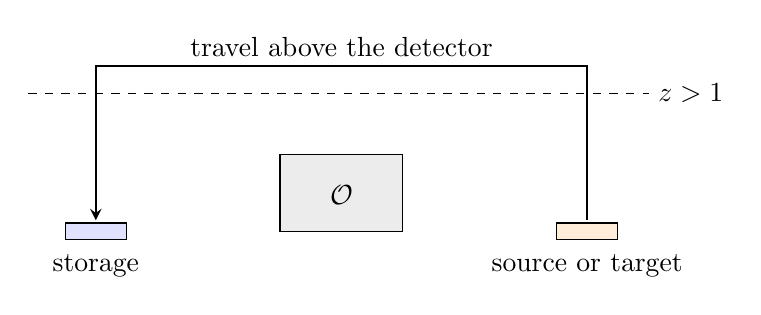
\begin{tikzpicture}[x=0.78cm,y=0.70cm,>=stealth]
 \draw[fill=gray!15] (4,0) rectangle (6,1.4);
 \node at (5,.65) {$\mathcal O$};
 \draw[fill=blue!12] (.5,-.15) rectangle (1.5,.15);
 \node[below] at (1,-.25) {storage};
 \draw[fill=orange!15] (8.5,-.15) rectangle (9.5,.15);
 \node[below] at (9,-.25) {source or target};
 \draw[->,thick] (9,.2)--(9,3)--(1,3)--(1,.2);
 \node[above] at (5,3) {travel above the detector};
 \draw[dashed] (-.1,2.5)--(10,2.5);
 \node[right] at (10,2.5) {$z>1$};
\end{tikzpicture}
\caption{Storage routing for a bounded detector, with the second
horizontal coordinate suppressed. All sources are evacuated before
any target is occupied. Scaling takes place at the storage positions;
horizontal travel takes place at height six. The drawing is schematic:
the storage and endpoint footprints are separated by the explicit
margins in Lemma~\ref{lem:sb-storage}.}
\label{fig:sb-storage}
\end{figure}

\subsection{Sheet and planar alternatives}
\label{subsec:sb-sheets}
When only a planar sheet carries the code, its vertical thickness can
be chosen after the horizontal motion. This allows a stronger path
statement: every horizontal coordinate of a tracked point can be made
a convex combination of its own endpoints. The widths in the two
horizontal directions need neither agree nor have equal products.  For source and target horizontal centers $a_i,b_i$ and half-widths $r_{ik}^0,r_{ik}^1$, interpolate the center and both half-widths by the same parameter $s$:
\[
 c_{i,\mathrm{hor}}=(1-s)a_i+sb_i,\qquad
 r_{ik}=(1-s)r_{ik}^0+sr_{ik}^1.
\]
Take starting height $z_0=1/4$ and private heights $z_i=1/2+i/(4(N+1))$.  Lift, interpolate, and lower on disjoint time stages.  A point of fixed fractional horizontal coordinates follows the convex combination of its own two endpoints.  The affine generator is
\[
 c_i'(t)+\operatorname{diag}\left(\frac{r'_{i1}}{r_{i1}},
 \frac{r'_{i2}}{r_{i2}},-\frac{r'_{i1}}{r_{i1}}-\frac{r'_{i2}}{r_{i2}}\right)(x-c_i(t)).
\]
This is exactly the reciprocal-normal-strain construction in Lemma~\ref{lem:sa-sheet-routing}, applied inside the open unit cube to the stated rectangles.  To verify its chart hypothesis for rectangles elsewhere than $[1/4,3/4]^2$, take one tenth of the minimum of $1$, the actual endpoint chart margins, the horizontal sup-norm gaps in the two endpoint families, and the private-height gaps.  The expanded plates then remain inside the cube and are separated by footprints during lift and lowering, and by height during interpolation.  The proof of that lemma consequently applies without a coordinate or viscosity normalization.

An invariant-plane realization solves a different problem. We first
allow the planar field to compress the rectangles to small squares,
route the squares through parking positions, and expand at the targets.
The lift will cancel its divergence in the normal direction.
For planar routing we use Lemma~\ref{lem:sa-planar-routing} with $D=(0,1)^2$ and the safe rectangle $G=(0,1/2)\times(0,1)$, or the right half of $D$ as specified below.  There are several explicit choices of the same finite path construction.  They preserve the full-rectangle affine maps but have their own smooth paths:
\begin{enumerate}
\item For the frontier sine plane, use initial contraction on $[0,1/4]$, $4N$ successive segment intervals on $[1/4,3/4]$, and expansion on $[3/4,1]$.  The contraction factors are $1-s+s\epsilon/r_{ik}$, and the expansion factors $1-s+sr'_{ik}/\epsilon$.  To avoid $l$ forbidden lines, select a vertex among $2l+3$ rational points $(a,1/4+a^2)$, $1/8<a<1/4$, also avoiding the two endpoints.  A line contains at most two such points.  Positive segment clearances give $\epsilon$ with moving and stationary squares separated by more than $10\epsilon$.
\item For the previous-tag plane, use $4N+2$ equal stages and logarithmic contraction and expansion.  Parking points have height half the minimum of all source and target center heights and abscissas $i/(2(N+1))$.  A two-segment vertex can be chosen below the finitely many forbidden rational lines: choose an abscissa below all positive vertical forbidden abscissas, then an ordinate below all positive intersections at that abscissa.  Include the line through the two endpoints among the exclusions.  With $\epsilon$ one hundredth of the minimum of $1$, side lengths, boundary margins, and squared line distances, $100\epsilon\le\min(1,d^2)\le d$.  A radial translation cutoff equal to one out to radius $2\epsilon$ and zero past $3\epsilon$ therefore misses every other tiny square of radius at most $\sqrt2\epsilon$.
\item For the shifted-start plane, choose all intermediate vertices in the right half.  A horizontal line below every endpoint and obstacle cannot coincide with any forbidden endpoint-obstacle line; avoiding their finitely many intersections gives a rational vertex.  Logarithmic contraction and expansion, with tiny half-side $\epsilon\le1/100$ and clearances greater than $10\epsilon$, keep a nonhalting point at first coordinate greater than $1/2-\epsilon>1/3$.
\item For the separator sine plane, use moving centers $c_i$ and half-size matrices $M_i$ throughout all stages, with linear interpolation during shrink and expansion.  Relative padded boxes $c_i+\lambda M_i[-1,1]^2$ are disjoint, and the field is
\[
 \sum_i\psi(M_i^{-1}(X-c_i))
     [c_i'+M_i'M_i^{-1}(X-c_i)].
\]
Here $\lambda=1+d_0/4$ with $d_0$ a positive endpoint margin/gap bound.  If $d_1$ bounds required boundary margins and $d_2\le1$ bounds the positive squared center separations along all planned segments, choose
$\epsilon=\tfrac12\min(m_0,d_1/\lambda,d_2/(4\lambda))$, with $m_0$ the minimum half-side.  Then padded tiny squares do not intersect, since their intersection would force center distance at most $2\sqrt2\lambda\epsilon<d_2$.  The path $c_i+M_i v$ is exact for every $v\in[-1,1]^2$.
\item For the two-cell-frontier plane, choose intermediate vertices on
$(1/8+r/8,1/8+r^2/8)$, $0<r<1$.  If there are $l$ forbidden lines, including the vertical lines through both endpoints, the $2l+1$ samples $r=j/(2l+2)$ include an admissible vertex.  A line intersects the parabola in at most two points.  Linear contraction and expansion and the one-hundredth clearance choice again prove full-rectangle transport and safe-region confinement.
\item For the zero-blank plane, choose a rational abscissa avoiding endpoint abscissas and vertical forbidden lines, then a rational ordinate avoiding the remaining line intersections.  Use fixed source/target cutoffs, linear contraction and expansion, and tiny half-side $\epsilon=d_*/10$, where $d_*$ is the minimum of $1$, half-sides, boundary margins and positive squared segment-to-obstacle distances.  Actual distances are at least $d_*$, while support and stationary-square radii sum to $3\sqrt2\epsilon<d_*$.  This includes boundary code points.
\end{enumerate}
In every case the first round moves all source centers to distinct parking positions before the second round occupies targets.  The cutoff equals one on a positive neighborhood of each tracked rectangle, or can be chosen with an arbitrarily smaller positive plateau collar without changing the field on that rectangle.  The exact formulas for the finite affine stages then apply on a positive initial neighborhood.  The stage fields vanish near stage endpoints, so they concatenate smoothly.  These verifications explain precisely why the planar-routing lemma applies to all the listed variants; no abstract extension of an unspecified code map is being assumed.

For the trigonometric variants put
\[
 U(X,z,t)=\left(\cos(2\pi z)b(X,t),
       -\frac{\sin(2\pi z)}{2\pi}\operatorname{div}_X b(X,t)\right).
\]
For the compact vertical variants use instead
\[
 U=(h'(z)b,-h(z)\operatorname{div}_X b),\qquad
 h(z)=(z-1/2)\chi(z),
\]
where $\chi=1$ on $[3/8,5/8]$ and is supported in $[1/4,3/4]$, periodically extended.  Lemma~\ref{lem:sa-invariant-lift} proves divergence cancellation, mean zero, and the exact planar motion on $z=0$ or $z=1/2$, respectively.  The same formula applies to a spatially constant planar loading field: its divergence is zero, and the horizontal mean vanishes after multiplication by $h'$.  Thus such loading does not need an unsupported compact planar chart assumption.

\section{Initialization and fixed observation regions}
\label{sec:sb-events}
A correct time-one instruction map does not yet prove a halting event.
We must locate the initial code, make the particle reach it from a fixed
label, and exclude the detector during every intermediate motion of a
nonhalting computation. We now prove
Theorem~\ref{thm:sb-realizations} by giving the actual placement and
checking the event for each of its rows.

\begin{proof}[Proof of Theorem~\ref{thm:sb-realizations}]
We specify the geometric data and check the all-time events in three groups.  Whenever one halting patch is specified, first merge the halting states as allowed above; this preserves the event, including initial halting.  The positive digit gaps remain valid at every closed rectangle edge.
In every case equation~\eqref{eq:sb-coded-map} makes the time-one map equal to the complete symbolic rule on its entire prefix rectangle.  For boxes and moving sheets, the stated affine formula holds on a three-dimensional neighborhood. For an invariant-plane construction, planar routing gives the formula on a planar neighborhood, and the lift reproduces that motion exactly on its invariant plane; no prescribed affine map off that plane is inferred.  Smooth flat collars allow the chosen pulse to be repeated every unit interval while preserving $U(0)=0$.

\emph{Euclidean full boxes.}
For left-word boxes use Lemma~\ref{lem:sb-postlog} with initial stacks $\#^\infty,w\square^\infty$, the odd-digit base $2m+2$, and state offsets $o_s$ given by distinct positive multiples of $3$ for nonhalting labels and distinct negative multiples for halting main labels.  The spatial code is $(o_s+c(L),c(R),0)$.  Use the relative-padding private-height construction following Lemma~\ref{lem:sb-boxes}, and load the rational initial code from the origin by a localized straight translation during $[0,1]$.  A cutoff with a unit-box plateau and a larger compact support suffices.  At a halt the first coordinate is at most $-2$.  On every nonhalting instruction both endpoint centers have first coordinate at least $3$, while the first half-width is at most $1/2$ throughout the period.  The entire path is therefore positive in that coordinate.  A nonhalting loading segment is nonnegative.  This proves the first row.

For right-word boxes use Lemma~\ref{lem:sb-rightword}, even digits in base $2m$ with blank digit zero, offsets $-2j$ for the $j$th halting state and $2j$ for the $j$th other state, both numbered from $1$.  The initial code is $(o_{q_0},b(w\square\#),0)$.  The full-box data have unit source half-height and reciprocal target half-height, and use exactly the additive-gap construction of Lemma~\ref{lem:sb-boxes}.  Initialize by the same lemma for one translated unit cube with all scales equal to one.  Its initial and final centers have height zero, although the loading path rises and descends; its first coordinate still interpolates from zero to the initial code.  Halting gives first coordinate at most $-1$.  Nonhalting rule centers are at least $2$ and half-widths at most $1/2$, excluding $x_1<-1/2$ at all times.

For tagged storage use Lemma~\ref{lem:sb-tagged}, digits $1,4,\ldots,3m-2$ in base $3m$, and offsets $o_s=3\operatorname{index}(s)$ with the halting main state indexed zero.  Use the thin boxes and $7N$-slot storage pulse of Lemma~\ref{lem:sb-storage}.  Load from $(-4,0,0)$ by three localized translations through
\[
 (-4,0,0),\quad(-4,0,6),\quad a_{\rm in}+(0,0,6),\quad a_{\rm in}.
\]
Take unit-box plateaus and margin $1/4$ for these loading pulses.  A nonhalting initial code has first coordinate at least $3$, so the vertical loading legs are outside the observation box and the horizontal leg is at height $6$.  The storage lemma excludes it on every later nonhalting period.  At a halting code both horizontal coordinates belong to $(0,1)$ and the height is zero, so the code lies strictly inside the observation box.

For boot-window prisms use Lemma~\ref{lem:sb-window}, base $2m+2$ with even digits and $d(E)=0$, offset $2$ for the halting main state, and distinct negative offsets $-3k$ for all others, with boot offset $-3$.  The initial code is exactly $(-3,0,0)$.  Include the boot rule in the full-box pulse, using the private heights $4(R+1)i$ and padding specified above.  Thus there is no loading interval outside the period.  Halting codes have first coordinate in $[2,3]$.  Every nonhalting endpoint footprint lies at first coordinate at most $-2$; the center interpolation and half-width bound keep the whole moving box strictly negative.  This proves the four Euclidean rows, including the initial-halt cases at time $1$ after loading or boot.

For tagged storage, uniqueness also holds under the pointwise comparison bounds
\[
 u,\partial_tu,\nabla u,\nabla^2u,p,\nabla p
       =O((1+|x|)^{-2})
\]
uniformly on every finite time interval, with pressure decaying at infinity.  Smoothness and these bounds imply the Sobolev and time-continuity requirements of Section~\ref{sec:model} by dominated convergence; $\partial_tu\in C_tL^2$ gives $C_t^1L^2$.  Hence the stated uniqueness includes this entire comparison class.  For the other Euclidean rows, a pressure representative in $C_tH^1$, modulo spatial constants when applicable, is the normalization specified in the theorem.  The constructed compactly supported velocity and zero pressure satisfy all these conventions.

\emph{Reserved-loader sheets.}
Both sheet rows use the post-update processor of Lemma~\ref{lem:sb-postlog}, with an additional history symbol $h_*$ unused in any ordinary rule.  For the left reserved sheets, place the halting interval at $[5/32,7/32]$ and enumerate the $J$ other states by $j=0,\ldots,J-1$ with intervals
\[
 [1/2+(3j+1)/(12J),\ 1/2+(3j+2)/(12J)].
\]
Use second interval $[1/4,3/4]$ and height $1/4$.  The input target is the code in $U_{q_0}$ of
$\#h_*\#^\infty,\diamond w\square^\infty$.
It lies in the interior of the unused image cylinder with prefixes $(\#h_*,\diamond)$.  Indeed the incoming $U_{q_0}$ images have left prefix $c\in A$ or $\#h_i$, never $\#h_*$.  A rational square centered at this target, with half-side half its minimum coordinate distance to the four cylinder edges, is therefore disjoint from every ordinary target.  Add a source square centered at $(1/2,1/2)$ with half-side half the minimum of $1/4$ and its positive distances in the first coordinate to the state intervals.  This source is disjoint from every ordinary source.  The positive affine source-to-target map supplies a loader in the same repeated pulse.

For the right reserved sheets, use the same table with history tail $h_*\square^\infty$, halting interval $[13/16,7/8]$, second interval $[1/4,1/2]$, and height $1/4$.  If $S$ is the number of other labels, put $\delta=1/(8(S+1))$ and give label $l=1,\ldots,S$ the first interval
\[
 [1/8+2(l-1)\delta,\ 1/8+(2l-1)\delta].
\]
These lie strictly below $3/8$.  The loader source is the square at $(1/2,1/8)$ with half-side $1/32$.  Its target is the code of $(U_{q_0},\#h_*\square^\infty,\diamond w\square^\infty)$, surrounded by the same half-minimum-margin square inside its reserved cylinder.  The same prefix argument proves separate disjointness of both enlarged instruction families.

Apply the moving-sheet construction to each placement.  The reciprocal normal strain is trace-free, all supports lie in the unit cube, and each horizontal coordinate of a tracked sheet point is a convex combination of its own endpoints.  At integer time $1$ the fixed particle is at its reserved $U$-code, and at time $2$ the ordinary marker-removal instruction gives the initial main configuration.  A machine halting initially is therefore detected at $2$.  Otherwise the main times satisfy
$t_0=2$, $t_{j+1}=t_j+2|L_{j+1}|+3$.
For the left placement, loading and all nonhalting endpoints lie at first coordinate at least $1/2$, and subsequent state intervals are in $(1/2,3/4)$.  For the right placement the loading point has coordinate $1/2$ and all nonhalting state intervals are below $3/8$.  Convex interpolation excludes the corresponding observation arcs throughout every period.  Halting state intervals are strictly inside the displayed arcs.  Periodicity starts at zero because the same loader is present in every pulse, with no image collision.

\emph{Invariant-plane realizations.}
For the frontier sine plane use Lemma~\ref{lem:sb-frontier}, its two-stack conversion, and odd digits in base $2m+1$.  With $P$ the auxiliary label set, put $s=1/(8|P|)$ and choose an index $i(p)\in\{0,\ldots,|P|-1\}$ for each label.  Use state squares with lower-left corners
\[
 o_p=(1/8+2s i(p),1/2)\quad(p\ne B_H),\qquad
 o_{B_H}=(3/4,1/2),
\]
and side $s$.  Nonhalting squares lie in $0<x_1<3/8$; the halt square lies in $[3/4,7/8]$.  Use the first planar routing choice above and the sine lift.  Load the rational initial code from $(1/2,1/4)$ along its straight segment, using a translated square cutoff with plateau half-side $1/32$ and support half-side $1/16$.  Both endpoints have chart margins at least $1/8$.  Nonhalting loading has first coordinate at most $1/2$, and every later nonhalting rectangle path remains in the left half.  Thus the event is exact.  The main checkpoint times are
\[
 t_0=1,\qquad t_{n+1}=t_n+2(2+n-h_{n+1})+4.
\]

For the previous-tag plane use Lemma~\ref{lem:sb-prelog} and odd digits in base $2m+1$.  Let $r=c(\square^\infty)$ and place the input rectangle at
\[
 [1/8-r/16,1/8-r/16+1/16]\times
 [1/4-r/8,1/4-r/8+1/8].
\]
Thus the two blank stacks have code exactly $(1/8,1/4)$.  Halting $B$-labels have disjoint first intervals inside $(2/3,5/6)$; all other noninput labels have them inside $(1/4,1/2)$, with common second interval $[1/4,1/2]$.  To place $n$ labels in $(a,b)$, take interval $[a+(2j-1)d,a+2jd]$, $j=1,\ldots,n$, $d=(b-a)/(2n+1)$.  Use the logarithmic planar shrink and expansion of the second routing choice and the sine lift.  The loader is already a disjoint prefix rule, so period one begins at zero.  The first main time is $t_0=1$, and the next is $t_{j+1}=t_j+2|L_j|+4$.  Every rule whose source and target are both nonhalting, including the loader when its target is nonhalting, has both rectangles in the left half and stays there throughout its pulse.  Halting main rectangles lie inside the observation arc.

For the shifted-start plane, prepend a fresh nonhalting state $q_s$ which writes back the scanned symbol and stays while entering the original initial state.  Apply Lemma~\ref{lem:sb-frontier} to this enlarged table.  This fresh state is different from the halt state even if the original machine halts initially.  Compute the rational initial normalized stack coordinates $(\xi_0,\eta_0)$, using blank combined-symbol tails and a history frontier at $2$.  If $L$ is the number of auxiliary labels, set $\ell=1/(16(L+1))$.  Put the halt square at lower-left corner $(1/8,1/2)$, the fresh-start square at
\[
 (3/4,3/4)-\ell(\xi_0,\eta_0),
\]
and the other squares at $(1/2+(2k+1)\ell,1/2)$, $k=0,\ldots,L-3$, all of side $\ell$.  These are disjoint; the initial code is exactly $(3/4,3/4)$, independently of the input.  The ordinary nonhalting squares lie in $1/2<x_1<5/8$, the start square near $(3/4,3/4)$, and the halt square lies inside $0<x_1<1/3$.  Use the third routing choice, with the right half as the safe region and tiny half-side at most $1/100$, then the compact vertical lift about $z=1/2$.  Nonhalting paths have first coordinate greater than $1/3$ throughout.  The repeated field starts at zero and is periodic from zero, with no separate loader.  The extra initial machine transition is simulated in finitely many periods, so initial halting of the given machine is still detected.

For the separator sine plane use Lemma~\ref{lem:sb-postlog} with initial stacks $\#\square^\infty,w\square^\infty$.  The nonhalting state rectangles, indexed $j=1,\ldots,n$, are
\[
 [(3j-2)/(6n),(3j-1)/(6n)]\times[1/4,3/4],
\]
and the halting rectangle is $[2/3,5/6]\times[1/4,3/4]$.  Use odd digits in base $2m+1$, the moving-center/moving-cutoff fourth routing choice, and the sine lift.  A spatially constant planar pulse takes $(1/4,1/2)$ along the straight segment to the rational initial code during $[0,1]$.  Both endpoints lie in the left half when the initial state is nonhalting, so this loading is safe.  Thereafter nonhalting rectangles and their paths remain in the left half; a halt code enters $(1/2,1)$.  The main times are $1+\sum_{j=1}^k(2|L_j|+3)$.

For the two-cell-frontier plane use Lemma~\ref{lem:sb-neighbor}, odd digits in base $2m+2$, and its complete three-cell branch list.  If $N$ is the number of nonterminal auxiliary labels, set $\ell=1/(16(N+1))$, put their square origins at $(1/4+2i\ell,1/4)$, $i=0,\ldots,N-1$, and the terminal origin at $(3/4,1/4)$, all with side $\ell$.  All source squares belong to nonterminal labels and lie in the left half; the halt square lies strictly in the observation arc.  Apply the rational-parabola fifth routing choice and the sine lift.  A compact planar loading pulse takes $(1/8,1/8)$ to the initial code along its segment, with plateau half-side $1/64$ and support half-side $1/32$.  The chart margins make this legal, including when initially halted.  Nonhalting loading and all nonhalting branches remain in the left half.  The main checkpoint recurrence is
$t_0=1$, $t_{n+1}=t_n+2(2+n-h_{n+1})+2$.

Finally, for the zero-blank plane use Lemma~\ref{lem:sb-postlog}, initial stacks $\#\square^\infty,w\square^\infty$, and even digits in base $2m+1$ with blank digit zero.  The $N$ nonhalting state squares have centers $(j/(2(N+1)),1/2)$, $j=1,\ldots,N$, and half-side $1/(8(N+1))$.  The halting square has center $(13/16,1/2)$ and half-side $1/32$.  Apply the fixed-cutoff sixth planar routing choice, then the compact vertical lift about $z=1/2$.  The initial normalized code is rational even when on a prefix boundary.  A spatially constant planar translation loads it from $(1/4,1/2)$; that segment stays in the left half in a nonhalting run.  All subsequent nonhalting paths stay there as well, while the halt square lies strictly inside $(3/4,7/8)$.  The checkpoint count is again $2|L_j|+3$ per transition after loading.

For all rows, induction on individual instruction periods now gives the exact encoded auxiliary configuration at each integer boundary through the first halt, or indefinitely in a nonhalting run.  The processor lemmas group those samples into the stated machine checkpoints, each after a finite positive number of instructions.  In an infinite run the times tend to infinity, so the all-time exclusions just proved cover every time.  After reaching a halted code no further symbolic rule is needed; the smooth fluid motion continues globally.  The state rectangles and separated digit intervals recover every finite prefix of both words, hence the represented configurations and their recorded head displacements.

All geometry and initial codes are obtained by finite symbol manipulation and rational arithmetic.  Smooth switches, logarithms of positive rational scales, finite differentiations, and bounded-index periodization give effective mixed-derivative evaluation as in Section~\ref{sec:model}.  At no point does constructing or evaluating the force require knowing the successive rules selected by the marked point.  The finite pulse acts on every branch domain during every period.  The residual realization lemma proves the claimed Navier--Stokes solution and comparison uniqueness.  Compact support or spatial periodicity and the repeated finite pulse give uniform derivative and energy bounds.

For the solenoidal alternative in the separator sine-plane row, apply Proposition~\ref{prop:projection-l2} to its mean-zero residual force.  If $\Delta r=\operatorname{div}f$ and $\int r=0$, replace $f$ by $f-\nabla r$ and the pressure by $-r$.  In Fourier coordinates,
\[
 r_k(t)=-\frac{\widehat{\operatorname{div}f}(t,k)}{4\pi^2|k|^2},\qquad k\ne0,
 \qquad r_0=0.
\]
Integration by parts gives arbitrarily high inverse-power coefficient bounds for every requested time derivative.  The shell $\|k\|_\infty=l$ contains $24l^2+2$ modes, so sufficiently many spatial derivatives provide effective summable tails for every derivative of $r$.  The projection preserves period one after loading, mean zero, and bounded derivatives, and leaves the velocity and its event unchanged.
\end{proof}

\subsection{Logarithmic clocks for the compact box constructions}
\label{subsec:sb-clock}
The periodic forces above and the following decaying forces are separate choices.  A reparametrization changes speed, while preserving every point of the material trajectory.

\begin{proposition}[Logarithmic alternatives]\label{prop:sb-log}
For each of the left-word-box, right-word-box, and tagged-storage constructions, retain its fixed initial label and observation set.  There is also an effective smooth force of fixed compact spatial support in
$L^2([0,\infty)\times\mathbb R^3)$ with exactly the same halting event and zero initial velocity.  It and all its derivatives are bounded.  The velocity's spatial derivatives are $O((1+t)^{-1})$, and their first time derivatives are $O((1+t)^{-2})$, uniformly in space.  The force itself is $O((1+t)^{-1})$ uniformly in space. The viscosity
in this statement is the same fixed physical $\nu$ as before the time
change.
\end{proposition}
\begin{proof}
Write $U(s,x)$ for the chosen construction, including its loading
interval. It is periodic only after that interval, but all its derivatives
are uniformly bounded on the whole half-line. Put
\[
 s(t)=\log(1+t),\quad a(t)=(1+t)^{-1},\quad
 \widehat U(t,x)=a(t)U(s(t),x).
\]
It is smooth and effective and has the same spatial support.  Since $U(0)=0$, its initial velocity is zero.  For every spatial multi-index $\alpha$,
\[
 \partial_x^\alpha\widehat U=a(\partial_x^\alpha U)\circ s,
 \qquad
 \partial_t\partial_x^\alpha\widehat U
   =a'(\partial_x^\alpha U)\circ s
       +a^2(\partial_s\partial_x^\alpha U)\circ s.
\]
The uniform derivative bounds for the original finite pulse give the stated spatial and first-time estimates.  Repeated chain and product rules express every higher mixed derivative as a finite sum of bounded derivatives of $U$ multiplied by derivatives of $a$ and $s$, so all are bounded as well.  The new residual force is exactly
\[
 \mathcal F_\nu[\widehat U]
  =a'U\circ s+a^2\big(\partial_sU+(U\cdot\nabla)U\big)\circ s
                -\nu a(\Delta U)\circ s.
\]
Its pointwise magnitude is at most $C(1+t)^{-1}$.  Fixed compact support gives a finite space-time square integral, since $\int_0^\infty(1+t)^{-2}\,dt<\infty$.  The same realization and uniqueness argument applies.  If $X(s)$ was the original material path, then $X(s(t))$ solves the new particle ODE by the chain rule.  The clock is increasing and maps $[0,\infty)$ onto itself, so the two paths have identical images and exactly the same observation event.  A checkpoint at original time $s_j$ is reached at the finite new time $e^{s_j}-1$; no finite upper bound on the halting time is required to prescribe this clock.
\end{proof}
